%%% LaTeX Template: Two column article
%%%
%%% Source: http://www.howtotex.com/
%%% Feel free to distribute this template, but please keep to referal to http://www.howtotex.com/ here.
%%% Date: February 2011

%%% Preamble
\documentclass[	DIV=calc,%
							paper=a4,%
							fontsize=11pt,%
							twocolumn]{scrartcl}	 					% KOMA-article class

\usepackage{lipsum}													% Package to create dummy text

\usepackage[english]{babel}										% English language/hyphenation
\usepackage[protrusion=true,expansion=true]{microtype}				% Better typography
\usepackage{amsmath,amsfonts,amsthm}					% Math packages
\usepackage[pdftex]{graphicx}									% Enable pdflatex
\usepackage[svgnames]{xcolor}									% Enabling colors by their 'svgnames'
\usepackage[hang, small,labelfont=bf,up,textfont=it,up]{caption}	% Custom captions under/above floats
\usepackage{epstopdf}												% Converts .eps to .pdf
\usepackage{subfig}													% Subfigures
\usepackage{booktabs}												% Nicer tables
\usepackage{fix-cm}													% Custom fontsizes
 \usepackage{amsmath}
 \usepackage{amssymb}
\usepackage{graphicx}

%%% Custom sectioning (sectsty package)
\usepackage{sectsty}			% Custom sectioning (see below)
\allsectionsfont{%			% Change font of al section commands
	\usefont{OT1}{phv}{b}{n}%	% bch-b-n: CharterBT-Bold font
	}

\sectionfont{%				% Change font of \section command
	\usefont{OT1}{phv}{b}{n}%	% bch-b-n: CharterBT-Bold font
	}



%%% Headers and footers
\usepackage{fancyhdr}			% Needed to define custom headers/footers
	\pagestyle{fancy}		% Enabling the custom headers/footers
\usepackage{lastpage}	

% Header (empty)
\lhead{Project Proposal}
\chead{}
\rhead{}
% Footer (you may change this to your own needs)
\lfoot{\footnotesize E: r.p.collins@sheffield.ac.uk, M: 07957 201954}
\cfoot{}
\rfoot{\footnotesize page \thepage\ of \pageref{LastPage}}	% "Page 1 of 2"
\renewcommand{\headrulewidth}{0.0pt}
\renewcommand{\footrulewidth}{0.4pt}



%%% Creating an initial of the very first character of the content
\usepackage{lettrine}
\newcommand{\initial}[1]{%
     \lettrine[lines=3,lhang=0.3,nindent=0em]{
     				\color{Black}
     				{\textsf{#1}}}{}}



%%% Title, author and date metadata
\usepackage{titling}				% For custom titles

\newcommand{\HorRule}{\color{DarkBlue}%	% Creating a horizontal rule
				\rule{\linewidth}{2pt}%
		      }
%%begin novalidate
\pretitle{\vspace{-30pt} \begin{flushleft} \HorRule 
				\fontsize{40}{40} \usefont{OT1}{phv}{b}{n} \color{Blue} \selectfont 
				}
\title{In Pipe Repair of PE Pipe by Friction Stir Welding}	

\posttitle{\par\end{flushleft}\vskip 0.5em}

\preauthor{\begin{flushleft}\large \lineskip 0.5em \usefont{OT1}{phv}{b}{sl} \color{DarkBlue}}
\author{Dr Richard Collins, }											% Author name goes here
\postauthor{\footnotesize \usefont{OT1}{phv}{m}{sl} \color{Black} 
					University of Sheffield, Sheffield Water Centre 								% Institution of author
					\par\end{flushleft}\HorRule}
%%end novalidate
\date{}																				% No date



%%% Begin document
\begin{document}
\maketitle
\thispagestyle{fancy} 			% Enabling the custom headers/footers for the first page 
% The first character should be within \initial{}

\initial{A} \textbf{significant cost of the repair of leaking pipes is in the locating and digging down to the level of the pipes.  
In addition due to the associated disruption, typically to road traffic, a solution that allows the repair of pipes that doesn't require digging would be a great advantage.  This proposal offers a design to allow the repair of PE pipes from inside the pipes, traversing from existing access points. By combining with existing sensing techniques it will allow the precise locating of leaks and assessment of the failure. In addition it will allow the post-installation verification and reassurance of joint viability, (both end joints and Top-Ts) , a common cause of failure.}





\section*{Problem}
Plyethelyene (PE) is the material of choice for the majority of pipe replacements due to its robustness and ability to install over long lengths. 
In general it suffers from a very low rate of failure compared to other materials. 
However there exists clear evidence that there is significant leakage in MDPE mains laid by the UK water industry.
In 2010 UKWIR \cite{UKWIR2010} reported electro-fusion jointing as the predominant cause of joint failure on PE mains with a calculated failure rate of between 3 and 4 failures per 100 km per year. 
More recent data is hard to come by there is a widely held view within the industry that failure rates on PE mains have not reduced there is still a significant problem.



\section*{Proposed Solution}
The proposed solution technique involves developing a smart welding head that will be able to traverse along the inside of a pipe, detect and locate the leak or joint, and then weld the leak closed, or re-weld the joint using a Friction Stir Weld (FSW) process.

\subsection*{Leak / Joint location and Assessment}
Reference to the ATU project
Acuratley navigating in the pipe environment has been demonstrated at The University of Sheffield in the Assessing the Underworld Project \cite{}.

\subsection*{Friction Stir Welding}
Friction stir welding (FSW) is a solid-state joining process that uses a non-consumable tool to join two facing workpieces without melting the workpiece material \cite{mishra2005friction}. Heat is generated by friction between the rotating tool and the workpiece material, which leads to a softened region near the FSW tool. While the tool is traversed along the joint line, it mechanically intermixes the two pieces of material, and forges the hot and softened material by the mechanical pressure, which is applied by the tool, much like joining clay, or dough.


\begin{figure}[htp]
 \centering
 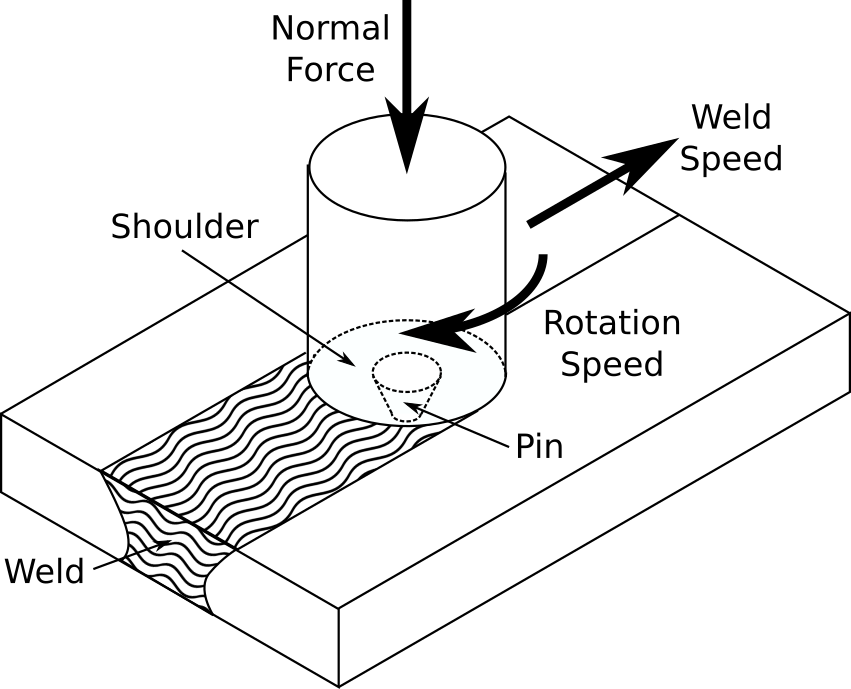
\includegraphics[width = 0.4\textwidth]{FrictionStirWeld}
 \caption{General friction stir welding process, the rotating tool (shoulder and pin) moves across the joint, mixing the material and forging with the frictional heat and pressure.}
 \label{FSWProcess}
\end{figure}

As can be seen in Figure \ref{FSWProcess} the working tool rotates and is passed across the required weld, the tool is comprised of two sections; the shoulder creates frictional heat, contains the softened material at the weld junction, and provides a suitable welding pressure,  the pin creates additional frictional head and directly stirs the materials together to form the weld.
Downward force is required to maintain the pressure on the joint and helps to create friction heat.


\subsubsection*{Friction Stir Welding of PE Pipes}
Whilst the majority of research into FSW has been undertaken on Aluminium and Steel, there have been a number of publications demonstrating its ability to join PE and other plastic sheets \cite{squeo2009friction,gao2014submerged}.  In PE the FSW process directly mixes the chains of the polymers and has been demonstrated to produce a very strong joint \cite{zafar2017friction}.


With FSW it is possible to weld both butted and lapped joints. As such it would be possible to fix leaks (butted joints), but also post installation re-weld an electro-fusion end joint (lapped and butted) or a Top-T (lapped) to confirm that the joint is secure. 

FSW sshould be possible in a full water pipe (it may even produce imporoved weld results \cite{gao2014submerged}

\begin{figure}[htp]
 \centering
 
 \caption{Section across an electro-fusion joint}
\end{figure}

\section*{Project Requirements}
The FSW process is established for their

The project 
It is proposed that the project would require to investigate:
\begin{itemize}
 \item optimal Geometry of tool (shoulder and pin)
 \item optimal tool rotational speed, downward pressure to maximise the weld speed and strength
\end{itemize}


The project is ideally 

\bibliographystyle{unsrt}
{\footnotesize
\bibliography{FSW}}



\end{document}